%%%%% Basic setup for one-sided printing:
%%%%% Margins: left 40mm, right 25mm, top and bottom 25mm (but beware, LaTeX adds 1in by itself)
%%%%% ---------------------------------------------------------------
\documentclass[12pt, a4paper]{report}
\usepackage{geometry}
\setlength\textwidth{145mm}
\setlength\textheight{247mm}
\setlength\oddsidemargin{15mm}
\setlength\evensidemargin{15mm}
\setlength\topmargin{0mm}
\setlength\headsep{0mm}
\setlength\headheight{0mm}
\newcommand{\openright}{\clearpage}

%%%%% Base setup for two-sided printing:
%%%%% ---------------------------------------------------------------
% \documentclass[12pt, a4paper, twoside, openright]{report}
% \setlength\textwidth{145mm}
% \setlength\textheight{247mm}
% \setlength\oddsidemargin{15mm}
% \setlength\evensidemargin{0mm}
% \setlength\topmargin{0mm}
% \setlength\headsep{0mm}
% \setlength\headheight{0mm}
% \let\openright=\cleardoublepage

%%%%% Czech language settings
%%%%% ---------------------------------------------------------------
% \usepackage[czech]{babel}
% \ifx\uv\undefined\newcommand{\uv}[1]{,,#1``}\fi

%%%%% Preamble with settings and macros
%%%%% ---------------------------------------------------------------
%%%%% Setting the input encoding of the files: UTF-8
%%%%% ---------------------------------------------------------------
\usepackage[utf8]{inputenc}

%%%%% Setting the language of the document
%%%%% ---------------------------------------------------------------
\usepackage{setspace}
\onehalfspacing
\usepackage{indentfirst}
\setlength{\parindent}{0pt}
\setlength{\parskip}{0.75\baselineskip}

%%%%% Color definitions
%%%%% ---------------------------------------------------------------
\usepackage{xcolor}
\definecolor{unicorn_blue}{HTML}{0B2A70}
\definecolor{unicorn_blue_light}{HTML}{40C8D3}
\definecolor{chart1}{HTML}{2D7DD2}  % Clear Blue
\definecolor{chart2}{HTML}{6C969D}  % Golden Yellow
\definecolor{chart3}{HTML}{97CC04}  % Lime Green
\definecolor{chart4}{HTML}{EEB902}  % Orange
\definecolor{chart5}{HTML}{474647}  % Dark Gray
\definecolor{chart6}{HTML}{F45D01}  % Steel Blue
\definecolor{chart7}{HTML}{9B6B6C}  % Dusty Rose
\definecolor{chart8}{HTML}{556F44}  % Forest Green

%%%%% Setting the color boxes/frames
%%%%% ---------------------------------------------------------------
\usepackage{tcolorbox}
% gray box preset
\newtcolorbox{gray-box}[1]{colback=gray!5!white,colframe=gray!50!black,title=#1}
\newtcolorbox{blue-box}[1]{colback=unicorn_blue!5!white,colframe=unicorn_blue,title=#1}


%%%%% Setting the colors and syntax of the code
%%%%% ---------------------------------------------------------------
% TODO: Define the colors
\usepackage{fvextra}
\usepackage{colortbl} % for colored rows/columns
\definecolor{codekeyword}{rgb}{0.0,0.3,0.7}
\definecolor{codestring}{rgb}{0.4,0.4,0.8}
\definecolor{codecomment}{rgb}{0.2,0.2,0.2}
\definecolor{codejsdoc}{rgb}{0.4,0.4,0.4}
\definecolor{codelinenum}{rgb}{0.8,0.8,0.8}
\definecolor{lightyellow}{rgb}{255, 255, 224}

% minted package setup
\usepackage[outputdir=dist]{minted}
\setminted{
	frame=none,
	breaklines=true,
	fontsize=\footnotesize,
	tabsize=2,
	linenos,
	numbersep=5pt,
	xleftmargin=0pt,
	baselinestretch=1.2,
	style=friendly,
%   TODO: highlighting not working
	highlightcolor=\color{lightyellow},
	keywordstyle=\color{codekeyword},
	stringstyle=\color{codestring},
	commentstyle=\color{codecomment}\itshape,
	morecomment=[s][\color{codejsdoc}]{/**}{*/},
	numberstyle=\footnotesize\color{codelinenum}
}

% listings package setup
\usepackage{listings}
\lstset{
	basicstyle=\ttfamily,
	columns=fullflexible,
	frame=single,
	breaklines=true,
	showstringspaces=false,
	keywordstyle=\bfseries,
	commentstyle=\itshape\color{gray},
	captionpos=t
}

% wrap long URLs
\PassOptionsToPackage{hyphens}{url}

%%%%% Tables
%%%%% ---------------------------------------------------------------
\usepackage{tabularx}

%%%%% Additional useful packages
%%%%% ----------------------------------------------------------------
\usepackage{amsmath}
\usepackage{amsfonts}
\usepackage{amsthm}
\usepackage{bm}
\usepackage{graphicx}
\usepackage[labelfont=bf]{caption}
\newcommand{\sourceDefaultLabel}{Own creation}
\newcommand{\sourceLabel}{Source:}
\newcommand{\source}[1][\sourceDefaultLabel]{\caption*{\hfill\footnotesize{\sourceLabel~\textit{#1}}}}
\usepackage{psfrag}
\usepackage{fancyvrb}
\usepackage[numbers]{natbib}
\usepackage{usebib}
\usepackage{tikz}
\usepackage{bbding}
\usepackage{icomma}
\usepackage{dcolumn}
\usepackage{booktabs}
\usepackage{paralist}
\usepackage{float}
\usepackage{subcaption}
\usepackage{epigraph}
\newcommand\foreign[1]{\emph{#1}}
\usepackage{pdfpages}
\usepackage{nameref}
% will create a reference to a chapter, section, ... including the number and in bold
\renewcommand{\fullref}[1]{\textbf{\nameref{#1}}}

% utils
\newcommand{\todo}[1]{\newline\textcolor{red}{\textbf{TODO:} #1}\newline}
\newcommand{\note}[1]{\newline\textcolor{blue}{\textbf{NOTE:} #1}\newline}
\newcommand{\theEvent}{\textbf{The Event}}
\newcommand{\theOrganizer}{\textbf{The Organizer}}
\newcommand{\eg}{e.g.,}

% Formatting numbers
\usepackage{siunitx} % for number formatting
% configure siunitx for Czech number formatting
\sisetup{
	group-separator={,},
	group-minimum-digits=4,
	round-mode=places,
	round-precision=0,
	output-decimal-marker={.},
}
\newcommand{\fmtnum}[1]{\num{#1}}
\newcommand{\fmtnump}[2][2]{\num[round-mode=places, round-precision=#1]{#2}}
\newcommand{\fmtczk}[1]{\num{#1}~CZK}
\newcommand{\fmtczkp}[2][2]{\num[round-mode=places, round-precision=#1]{#2}~CZK}
% bold (using mathbf + textbf)
\newcommand{\bfmtnum}[1]{\boldmath\textbf{\num[reset-math-version=false]{#1}}}
\newcommand{\bfmtnump}[2][2]{\boldmath\textbf{\num[reset-math-version=false, round-mode=places, round-precision=#1]{#2}}}
\newcommand{\bfmtczk}[1]{\boldmath\textbf{\num[reset-math-version=false]{#1}~CZK}}
\newcommand{\bfmtczkp}[2][2]{\boldmath\textbf{\num[reset-math-version=false, round-mode=places, round-precision=#1]{#2}~CZK}}

% Command for color box indicator
\newcommand{\colorindicatorhex}[1]{%
	\textcolor[HTML]{#1}{\rule{0.8em}{0.8em}}\hspace{0.5em}%
}
\newcommand{\colorindicator}[1]{%
	\textcolor{#1}{\rule{0.8em}{0.8em}}\hspace{0.5em}%
}

%%%%% Setting the acronyms
%%%%% ---------------------------------------------------------------
\usepackage{acro}
\DeclareAcronym{api}{short=API,     long=Application Programming Interface }

%%%%% Setting the headings
%%%%% ------------------------------------------------------------
\usepackage{titlesec}
%\titlespacing*{\chapter}{0pt}{-10mm}{5mm}
\titleformat{\chapter}{\normalfont\huge\bfseries}{\thechapter}{1em}{}

%%%%% Counters and questions
%%%%% ------------------------------------------------------------
\usepackage{totcount}
\usepackage{xparse}
% counter for questions
\newcounter{rqcounter}
\regtotcounter{rqcounter}

% Configure autoref format for research questions
\makeatletter
\def\therqcounter{\@arabic\c@rqcounter}
\@addtoreset{rqcounter}{chapter}
\def\autoref@rqcounter#1{\RQ{#1}}
\def\RQ#1{\textup{RQ#1}}
\makeatother

% Command to define a new research question
\NewDocumentCommand{\defresearchq}{m m}{
	\refstepcounter{rqcounter}
	\expandafter\edef\csname rqnum:\string#1\endcsname{\therqcounter}
	\expandafter\label\expandafter{rq:#1}
	\expandafter\newcommand\csname rq:\string#1\endcsname{
		\textbf{\csname rqnum:\string#1\endcsname:} #2
	}
}

% Command to use a research question
\NewDocumentCommand{\researchq}{m}{
	\hyperref[rq:#1]{\csname rq:\string#1\endcsname}
}

\renewcommand{\therqcounter}{RQ\arabic{rqcounter}}

%%%%% Hyperlinks setup
%%%%% ------------------------------------------------------------
\usepackage[unicode]{hyperref}
\hypersetup{pdftitle=Cashless festival data analysis and analytical dashboard development,
    pdfauthor=Bc. Filip Ditrich
    ps2pdf,
    colorlinks=true,
    urlcolor=black,
    linkcolor=black,
    citecolor=black,
    pdfstartview=FitH,
    pdfpagemode=UseOutlines,
    pdfnewwindow,
    breaklinks
}

%%%%% Bibliography setup
%%%%% ---------------------------------------------------------------
\bibliographystyle{/Users/filipditrich/University/master_thesis/thesis/czplainnat.bst}
\renewcommand{\bibname}{References}

%%%%% Table of contents setup
%%%%% ---------------------------------------------------------------
\usepackage[nottoc]{tocbibind}
\renewcommand{\listingscaption}{Source code}
\renewcommand{\listoflistingscaption}{List of Source Codes}
\usepackage[titles]{tocloft}
\renewcommand\cftchapafterpnum{\vskip0pt}
\renewcommand\cftsecafterpnum{\vskip2pt}
\usepackage[toc,page]{appendix}
% \renewcommand{\appendixtocname}{Seznam příloh}
% \renewcommand{\appendixpagename}{Seznam příloh}

%%%%% Figures setup
%%%%% ---------------------------------------------------------------
\newcommand{\FIGDIR}{./figures}    %%% cesta do adresáře s obrázky

%%%%% TODO:
%% - [] setup the structure and technical setup
%% - [] add copy of the assignment PDF

%%%%% Main document part
%%%%% ------------------------------------------------------------
\begin{document}
%%% title page
    %%% Hard title page
%%%%%%% Wording: ⏳
%%%%%%% Styling: ⏳
%%%%%%% References: ⏳
%%%%% Grammar: ⏳
%%% --------------------------------------------------------------
\pagestyle{empty}
\begin{center}
{\Large\bfseries\MakeUppercase{Unicorn Vysoká škola s.r.o.}}
    \vfill

    {\Huge\bfseries\MakeUppercase{Master's Thesis}} \\

    \vfill

    \noindent\begin{minipage}{\textwidth}
                 \begin{Large}
                     \textbf{2024} \hfill \textbf{Bc. Filip \MakeUppercase{Ditrich}}
                 \end{Large}
    \end{minipage}
\end{center}
 % FIXME: remove
    %%% Cover page
%%%%%%% Wording: ⏳ (TODO: check for year 24 or 25)
%%%%%%% Styling: ✅
%%%%%%% References: ✅
%%%%% Grammar: ✅
%%% --------------------------------------------------------------
\pagestyle{empty}
\begin{center}

%%% school name
{\bfseries\large UNICORN VYSOKÁ ŠKOLA s.r.o.}

	\vspace{5mm}

	%%% název oboru
	{\Large Software Engineering and Big Data}

	\vfill
	\vspace{5mm}

	%%% logo
	\centerline{\mbox{
\includegraphics[width=83.3mm]{\CoreFigures/uu-icon}}}

	\vfill
	\vspace{5mm}

	%%% thesis type
	{\large\MakeUppercase{Master's Thesis}}

	\vspace{15mm}

	%%% name of the thesis
	{\LARGE\bfseries Cashless festival data analysis and analytical dashboard development}

	\vfill

	%%% author and supervisor
	\begin{tabular}{rl}
		Author:     & Bc.~Filip Ditrich       \\
		\noalign{\vspace{2mm}}
		Supervisor: & Mgr.~Václav Alt,~Ph.~D. \\
	\end{tabular}

	\vfill

	%%% rok
	Prague 2024

\end{center}

%%% TODO: copy of the assignment
%    \includepdf[pages={1}]{\FIGDIR/zadani-zp.pdf}
%    \includepdf[pages={2}]{\FIGDIR/zadani-zp.pdf}
%%% declaration
    %%% Statutory Declaration
%%%%%%% Wording: ⏳
%%%%%%% Styling: ⏳
%%%%%%% References: ⏳
%%%%% Grammar: ⏳
%%% --------------------------------------------------------------
\newpage
\pagestyle{empty}
\vspace*{\stretch{8}}

%%% title
\noindent
{\large\bfseries Statutory Declaration}\\

%%% text
\noindent
I hereby declare that I have written my Master's Thesis on the topic of \textit{Cashless festival data analysis and analytical dashboard development} by myself, under the guidance of my thesis supervisor, using only the technical publications and other information sources which are all quoted in the thesis and listed in the bibliography.
I declare that artificial intelligence tools have been used only for support activities and in accordance with the principle of academic ethics.

As the author of this Master's Thesis, I also declare that in association with its writing I have not violated the copyright of any third party or parties and I am fully aware of the consequences of provisions of s. 11 et seq. of Act No. 121/2000 Coll., the Copyright Act.\\

Furthermore, I hereby declare that the submitted hard copy of this Master's Thesis is identical to the electronic version I have submitted.\\

%%% signature - place/date
\vspace{18mm}
\noindent
In \makebox[4cm]{\dotfill} on \makebox[2.5cm]{\dotfill}
\hspace*{\fill}
\makebox[4cm]{\dotfill}

%%% signature
\begin{flushright}
	\noindent
	Bc.~Filip~Ditrich
\end{flushright}

%%% acknowledgements
    %%% Acknowledgements
%%%%%%% Wording: ⏳
%%%%%%% Styling: ⏳
%%%%%%% References: ⏳
%%%%% Grammar: ⏳
%%% --------------------------------------------------------------
\newpage
\pagestyle{empty}
\vspace*{\stretch{8}}

%%% title
\noindent
{\large\bfseries Acknowledgements}\\

%%% text
\noindent
I would like to express my sincere gratitude to my supervisor, Mgr. Václav Alt, for his guidance, support, and valuable advice throughout the process of writing this thesis. I would also like to thank my family and friends for their encouragement and understanding.

%%% first page
    %%% First page
%%%%%%% Wording: ⏳
%%%%%%% Styling: ⏳
%%%%%%% References: ⏳
%%%%% Grammar: ⏳
%%% --------------------------------------------------------------
\newpage
\pagestyle{plain}

%%% pagination start
\setcounter{page}{6}

%%% edges of the page
\newgeometry{textwidth=100mm, textheight=247mm, left=40.4mm, right=75mm}

%%% background
\tikz[remember picture,overlay]
\node[opacity=1,inner sep=0pt] at (current page.center)
	{
\includegraphics[width=\paperwidth,height=\paperheight]{\CoreFigures/side-banner}};

\begin{center}

	%%% logo
	\centerline{\mbox{
\includegraphics[width=39.6mm]{\CoreFigures/uu-icon}}}

	\vfill

	%%% thesis name in english
	\Large\textbf{Cashless festival data analysis and analytical dashboard development}

	\vspace{5mm}

	%%% thesis name in czech
%    \Large{Analýza dat bezhotovostního festivalu a vývoj analytického dashboardu}

	\vfill

	%%% logo
	\centerline{\mbox{
\includegraphics[width=45mm]{\CoreFigures/uu-logo}}}

\end{center}
\restoregeometry

%%% abstract
    %%% Abstract
%%%%%%% Wording: ⏳
%%%%%%% Styling: ⏳
%%%%%%% References: ⏳
%%%%% Grammar: ⏳
%%% --------------------------------------------------------------
\newpage
\pagestyle{plain}

%%% abstract in english
\nobreak\vbox to 0.49\vsize{
	\setlength\parindent{0mm}
	\setlength\parskip{3.5mm}

	%%% title
	{\large\bfseries Abstract}

	%%% text
	\noindent
	This thesis analyzes transaction data from a larger Czech festival that utilized the NFCtron payment system, addressing 29 research questions focused on cashflow, system performance, beverage consumption, and customer behavior.
	The analysis encompasses over~\fmtnum{141000} transactions from more than~\fmtnum{10000} unique attendees, providing comprehensive insights into the festival dynamics.

	Methodology ranged from establishing a local analysis environment and implementing data anonymization techniques to ensure privacy while maintaining analytical value to answering all research questions.
	Key insights about festival dynamics were revealed and resulted in an interactive analytical dashboard prototype developed to demonstrate the findings.

	While the dashboard remains in prototype stage, the analytical architecture and findings provide a foundation for future development and have already contributed to improvements in NFCtron's analytical capabilities.

	\textit{Keywords: festival data analysis, cashless payments, data visualization, data anonymization, interactive analytic dashboard, Python, Dash and Plotly}
	\vss}

%%% abstract in czech
\vbox to 0.5\vsize{
	\setlength\parindent{0mm}
	\setlength\parskip{5mm}

	%%% title
	{\large\bfseries Abstrakt}

	%%% text
	\noindent
	Tato práce analyzuje transakční data z většího českého festivalu, který využíval platební systém NFCtron, a zaměřuje se na 29 výzkumných otázek týkajících se pěněžních toků, výkonu systému, konzumace nápojů a chování zákazníků.
	Analýza zahrnuje přes~\fmtnum{141000} transakcí od více než~\fmtnum{10000} unikátních návštěvníků, poskytující komplexní pohled na dynamiku festivalu.

	Metodologie zahrnovala vytvoření lokálního analytického prostředí, implementaci technik anonymizace dat, které zajistily ochranu soukromí a zároveň zachovaly analytickou hodnotu, až po zodpovězení všech výzkumných otázek.
	Klíčové poznatky o dynamice festivalu byly odhaleny a vedly k vývoji prototypu interaktivního analytického dashboardu, který demonstruje jejich výsledky.

	Ačkoliv je dashboard stále ve fázi prototypu, analytická architektura a zjištění poskytují základ pro budoucí vývoj a již přispěly k zlepšení analytických schopností NFCtron.

	\textit{Klíčová slova: analýza dat z festivalu, bezhotovostní platby, vizualizace dat, anonymizace dat, interaktivní analytický dashboard, Python, Dash a Plotly}
	\vss}

%%% table of contents
    \newpage
    \pagestyle{plain}
    \tableofcontents
%%% chapters
    % chapter - introduction
    %%% Introduction
%%%%%%% Wording: ⏳
%%%%%%% Styling: ⏳
%%%%%%% References: ⏳
%%%%% Grammar: ⏳
%%% --------------------------------------------------------------
\chapter*{Introduction}
\addcontentsline{toc}{chapter}{Introduction}
\label{chap:introduction}


\section*{Background and Motivation}
\addcontentsline{toc}{section}{Background and Motivation}
\label{sec:introduction-background-motivation}
Payments at festivals are a crucial part of the successful event management.
The shift from cash to cashless payments has been a significant trend in the last decade that has brought many benefits to both festival organizers and attendees.

However, traditional cashless payment systems utilizing payment terminals are not only expensive to reliably implement at a venue, where the internet connection is often unreliable and requires expensive Base Transceiver Stations (BTS) set-ups or in-place wired/optical internet implemented which can cost up to several million CZK, but also do not provide any insights into the data generated by the transactions.
In the best case scenario, the organizers are able to generate a report of processed transactions made by each terminal.

Which, frankly, is not enough to make any actionable decisions based on the data.
Moreover, given the event organizers are not data scientists, they often lack the knowledge and tools to analyze the data and extract valuable insights from it.

That is where NFCtron comes in and offers a solution that not only provides a reliable cashless payment system, with credit-based NFC chip bracelets supporting offline mode or card terminal payment solutions, but also provides a comprehensive B2B platform that allows the organizers, the vendors and event the third-party partners to benefit from the data that the system operates with.

The system is a full-scope solution that provides from initial online ticket sales and online credit top-up, through attendee check-in, on-site credit top-up attendee access control, security monitoring, vendor sales and inventory management, most importantly the fast and reliable payment processing with the real-time data analytics and reporting, all the way to the post-event automatic settlement and reporting.

It simply provides everything an event organizer needs to successfully and efficiently manage their event without the need to worry about any technicalities or staff management.
Since NFCtron does not only provide the system as a service, but also provides experienced Event Managers, cashiers, check-in brigadiers and other staff to operate the system and the event itself ensuring that the organizer can focus on the event in terms of communication, marketing, line-ups and other important aspects of the event.

Put, NFCtron offers organizers a peace of mind and a guarantee that their event will be a success.

\subsection*{NFCtron Company}
\label{subsec:introduction-background-motivation-nfctron}
NFCtron is a Czech company that has been operating since around 2019.
In its early beginning during a COVID-19 pandemic was on the verge of survival because of the event industry being paralyzed by the government restrictions.
However, the company survived and even in these difficult times managed to turn the disadvantage into an advantage by focusing on the core system and product development.

Which years later resulted in a robust and reliable system.
It is now used by many event organizers across the Czech Republic and Slovakia and is currently expanding to other countries in Central Europe such as Austria, Poland and Germany.
In its primary market – the Czech Republic – NFCtron penetrated the market and is now the leading cashless payment system provider for festivals and other events.

In recent years, the company has also been focusing on expanding to the Payments market focusing both on Card Acquiring and Card Issuing.
From the acquiring part, it is now actively developing its own SoftPOS solution that will allow vendors to accept payments via mobile phones.
On the other hand, on the Issuing part, it is also working on Card Issuing; that will allow the company to issue its own NFCtron branded payment cards in cooperation with Mastercard.

A big part of the successful market penetration was the company's focus on the business-to-business (B2B) side of the business with event organizers.
Giving the organizers amounts of data improving their decision-making and providing them with insights allowing them to optimize their events.
And most importantly, providing them with economic aspects and cashflow optimizations that allows many events and festivals to survive and continue to operate.

\subsection*{Personal Position and Motivation}
\label{subsec:introduction-background-motivation}
I have been with the company from the COVID-19 times.
My current position is a Chief Product Officer (CPO), and I am responsible for the product development and the product management of all the products and services that NFCtron offers.
This allows me to have a deep insight into the system and most importantly, access to all the data that the system generates.
As previously mentioned, the company's success is based on the B2B side of the business and that means services and products provided to the event organizers.

The main product, that organizers have access to is the platform called \textbf{NFCtron Hub}.
My personal goal and personal motivation to work on this thesis is to discover new ways to improve the platform and provide even more valuable insights to the organizers.

\section*{Problem Statement}
\addcontentsline{toc}{section}{Problem Statement}
\label{sec:introduction-problem-statement}
Even though the system provides a lot of data, it still has a lot of potential to provide even more valuable insights to the organizers.
Currently, the previously mentioned B2B platform, \textbf{NFCtron Hub}, provides real time data analytics dashboard presenting the most important KPIs and metrics to the organizers.

These KPIs and metrics summarize:
\begin{itemize}
	\item \textbf{Total sales}: the total amount spent on online ticket sales and on-site payments.
	\item \textbf{Total sales in time}: the total amount above split into time intervals.
	\item \textbf{Total refunds}: the total number of sale reversals or refunds made including refunds from online tickets, refunds of on-site payments and chip credit refunds.
	\item \textbf{Chip balances}: the current balance topped-up on the NFC chip bracelets on-site or pre-topped-up online.
	\item \textbf{Customer orders rating}: customers can rate their orders via a NFCtron mobile application which provides the organizers with feedback on the vendor's performance and the quality of the products sold.
\end{itemize}

Moreover, it provides less clear data such as
\begin{itemize}
	\item \textbf{List of vendors}: the list of vendors presents at the event with their sales and rating.
	\item \textbf{List of products}: the list of products sold at the event with their sales and rating.
	\item \textbf{List of points of sale}: the list of selling points at the event with their sales and rating.
	\item \textbf{List of top-up places}: the list of top-up places at the event with the amount of top-ups made.
	\item \textbf{List of customer chips}: the list of unique individual NFC chips issued to the customers with their balance, spending and security status.
	\item \textbf{List of customer ratings}: the list of customer ratings with their feedback from points of sale.
\end{itemize}

And finally, it also provides unstructured data in the form of data exports in tabular format that can be used for further analysis:
\begin{itemize}
	\item \textbf{Product exports} – list of all products sold with summarized metrics.
	\item \textbf{Points of sale exports} – list of all selling points with summarized metrics.
	\item \textbf{Vendor exports} – list of all vendors with summarized metrics.
	\item \textbf{Deal exports} – list of summarized sales made under a deal\footnote{
		A deal is an arrangment between the organizer and the vendor that states the terms of the vendor's presence at the event, the products they are allowed to sell, the price of the products, the commission the vendor pays to the organizer and other terms of the deal.
	} Between the organizer and the vendor.
	\item \textbf{Transaction exports} – a heavy export of all transactions made at the event.
	\item \textbf{Ticket redeems exports} – list of all tickets redeemed at the event.
	\item \textbf{And other exports regarding the online sales} – list of all online ticket sales, top-ups, receipts, customers and other data.
\end{itemize}

With the above giving some initial picture about the capabilities of the system, the platform (and thus the organizers) still face several problems or challenges that need to be addressed:
\begin{enumerate}
	\item \textbf{Problem 1}: The main KPI metrics may provide some core insights, but the other less or unstructured data is not used to its potential.
	\item \textbf{Problem 2}: The organizers are not data scientists and need a simple and clear way to understand the data.
	\item \textbf{Problem 3}: Even with all this data, there is still a lot that can be done to dig deeper and provide more valuable insights.
\end{enumerate}

\section*{Objectives of the Work}
\addcontentsline{toc}{section}{Objectives of the Work}
\label{sec:introduction-objectives}
With the problems stated above, the main objective of this thesis is to analyze, answer and present results to important questions about the available data and the potential insights that can be extracted from it.

But to achieve this, it was a prerequisite to find a willing event organizer, that would provide the data and would be willing to cooperate on the project.
Cooperate in terms of providing valuable insights into what they would like to know more about their event.

\subsection*{In Cooperation with the Event Organizer}
\label{subsec:introduction-objectives-cooperation}
For this purpose, I have chosen a not more undisclosed event organizer, that has been a close and helpful partner of NFCtron for many seasons.
Together with the organizer in the first step, we have stated the following requirements to perform the analysis:
\begin{itemize}
	\item \textbf{Requirement 1}: The event and organizer should be kept undisclosed.
	\item \textbf{Requirement 2}: The data should be anonymized to not leak any possible sensitive information about vendors or customers.
\end{itemize}

The next step was to choose an event from which the data will be used.
As it cannot be disclosed any further, we will refer to the event as~\theEvent~and the organizer as~\theOrganizer.

Now the important information about~\theEvent~for this study is the following:
\begin{itemize}
	\item \theEvent~is a music festival that has been organized for several years now.
	\item \theEvent~takes place in the Czech Republic in the begging of July 2025.
	\item \theEvent~is a 3-day event with multiple stages and multiple vendors.
	\item \theEvent~uses NFCtron system for cashless payments and access control.
	\item \theEvent~had around 7,000 attendees in 2024 and had a roughly 43\% increase in 2025 to around 10,000 attendees.
\end{itemize}

\subsection*{Data Analysis Objectives}
\label{subsec:introduction-objectives-data-analysis}

The final step was to define questions or data analysis objectives that should be answered or achieved by the end of the thesis.

Together in the cooperation with~\theOrganizer~and several internal colleagues in NFCtron, we have defined the following questions for the data analysis:

\subsubsection*{Cashflow and Revenue}
\defresearchq{cashflow-total-revenue}{What was the total revenue of the organizer and what does it consist of?}
\defresearchq{cashflow-top-up-balance}{How much and by what means was the balance topped up on the chips?}
\defresearchq{cashflow-remaining-balance}{How much balance remained on all chips after the event and after refunds?}
\defresearchq{cashflow-total-sales}{What was the total sales of the event, how much of it was the sales of the organizer and how many external vendors?}
\begin{itemize}
	\item \textit{\researchq{cashflow-total-revenue}}
	\item \textit{\researchq{cashflow-top-up-balance}}
	\item \textit{\researchq{cashflow-remaining-balance}}
	\item \textit{\researchq{cashflow-total-sales}}
\end{itemize}

These questions should provide currently unclear insights into the cashflow and revenue sources of the event.
Possible answers to these questions could provide the organizer with valuable insights into the economic aspects of the event and could help optimize the cashflow and revenue sources for the next event.

\subsubsection*{Performance}
\defresearchq{performance-transactions}{How many transactions were processed in total and what was the largest "peak" in the volume of transactions processed by the system (and when)?}
\defresearchq{performance-processing-during-peaks}{What was the average transaction processing time during peak hours?}
\defresearchq{performance-delays-downtimes}{Were there any significant delays or downtimes in processing transactions?}
\defresearchq{performance-best-selling-points}{What were the best-selling points?}
\defresearchq{performance-best-top-up-points}{What were the best top-up points?}
\defresearchq{performance-best-vendors}{Who were the best vendors?}
\defresearchq{performance-best-products}{What were the best products?}
\begin{itemize}
	\item \textit{\researchq{performance-transactions}}
	\item \textit{\researchq{performance-processing-during-peaks}}
	\item \textit{\researchq{performance-delays-downtimes}}
	\item \textit{\researchq{performance-best-selling-points}}
	\item \textit{\researchq{performance-best-top-up-points}}
	\item \textit{\researchq{performance-best-vendors}}
	\item \textit{\researchq{performance-best-products}}
\end{itemize}

The current platform already provides some performance metrics, but these questions should provide more detailed insights into the performance of the event.

\subsubsection*{Beverage Consumption}
\defresearchq{beverage-total-consumption}{How much was the total consumption of drinks/fluids?}
\defresearchq{beverage-returnable-cups}{How many returnable cups were issued, and how many were returned or not returned?}
\defresearchq{beverage-popular-category}{What was the most popular drink category?}
\defresearchq{beverage-top-beer}{What was the TOP beer brand, how much was consumed and sold?}
\defresearchq{beverage-top-alcoholic}{What was the TOP brand of other alcoholic beverages, how much was consumed and sold?}
\defresearchq{beverage-top-non-alcoholic}{What was the TOP brand of non-alcoholic beverages, how much was consumed and sold?}
\begin{itemize}
	\item \textit{\researchq{beverage-total-consumption}}
	\item \textit{\researchq{beverage-returnable-cups}}
	\item \textit{\researchq{beverage-popular-category}}
	\item \textit{\researchq{beverage-top-beer}}
	\item \textit{\researchq{beverage-top-alcoholic}}
	\item \textit{\researchq{beverage-top-non-alcoholic}}
\end{itemize}

Currently, a more in-depth product analysis is missing in the platform and the most important part of the product sales analysis at festivals is the beverage consumption.
These questions should try to answer and give detailed insights into the beverage consumption, preferences and sales at the event.

\subsubsection*{Customers}
\defresearchq{customers-total-attendance}{What was the total attendance at the event, how many active customers were at the event each day?}
\defresearchq{customers-bank-cards}{What is the distribution of bank cards used to refund credit?}
\defresearchq{customers-card-schemes}{What is the distribution of card schemes used to top up credit on-site and online?}
\defresearchq{customers-new-visitors}{What was the course of the event in terms of new visitors and when were the largest "peaks"?}
\defresearchq{customers-visitor-time}{What is the average time of a visitor from arrival in the first transaction?}
\defresearchq{customers-top-up-peaks}{What was the course of the event in terms of topping up credit on-site and when were the largest "peaks"?}
\defresearchq{customers-top-up-more-than-once}{How many customers topped up credit more than once and how much only once?}
\defresearchq{customers-visitors-difference}{What was the difference between one-day, two-day and three-day visitors in terms of spending, topping up and refunded credit?}
\defresearchq{customers-visitors-types-difference}{What was the difference between spending and topping up between different types of visitors (primarily online vs.\ on-site)?}
\defresearchq{customers-drink-preferences}{What were the preferences for the type of drink throughout the day?}
\defresearchq{customers-common-combinations}{What were the most common combinations of products?}
\defresearchq{customers-top-up-online}{How many customers topped up credit in advance online?}
\defresearchq{customers-distribution-types}{What was the distribution of customers by their type (on-site, online, staff, guest, VIP)?}
\defresearchq{customers-mobile-app}{How many customers used the mobile application?}
\begin{itemize}
	\item \textit{\researchq{customers-total-attendance}}
	\item \textit{\researchq{customers-top-up-online}}
	\item \textit{\researchq{customers-distribution-types}}
	\item \textit{\researchq{customers-mobile-app}}
	\item \textit{\researchq{customers-bank-cards}}
	\item \textit{\researchq{customers-card-schemes}}
	\item \textit{\researchq{customers-new-visitors}}
	\item \textit{\researchq{customers-visitor-time}}
	\item \textit{\researchq{customers-top-up-peaks}}
	\item \textit{\researchq{customers-top-up-more-than-once}}
	\item \textit{\researchq{customers-visitors-difference}}
	\item \textit{\researchq{customers-visitors-types-difference}}
	\item \textit{\researchq{customers-drink-preferences}}
	\item \textit{\researchq{customers-common-combinations}}
\end{itemize}

The customer analysis is the most important part of the data analysis.
It is crucial for the festival organizers to know their customer base and their behavior to optimize the event and make it more attractive for the customers.

Currently, no customer analysis, other than the customer ratings and list of customer chips, is available in the platform.

Answering these questions will possibly lead to the most valuable insights about the event's customer base and their behavior that no other platform or system currently provides.

Making these questions crucial and most valuable for the organizer and for the platform itself.

\subsection*{Technical Objectives}
\label{subsec:introduction-objectives-technical}
Answering the above questions will require a technical solution that will be able to process the data and provide the answers.

The scope of this study is not to implement a new system or a new platform and not even to implement any new changes to the existing NFCtron Hub platform.
It is to find answers to the above questions and present them in a clear and understandable way in the form of a simple internal dashboard.

The technical goals of this study are:
\begin{itemize}
	\item Prepare, process and analyze the data from~\theEvent.
	\item Find answers to the above questions.
	\item Implement a simple internal dashboard that will present the answers to the questions.
\end{itemize}

\section*{Scope of the Study}
\addcontentsline{toc}{section}{Scope of the Study}
\label{sec:introduction-scope}
To ensure the feasibility and focus of the study, certain boundaries have been defined in terms of what is included and excluded from the scope of the study.

\subsection*{Included in the Scope}
\label{subsec:introduction-scope-included}
\begin{itemize}
	\item The study will focus on transactional, customer, and operational data from a specific event, referred to as~\theEvent.
	\item Key areas of analysis include cashflow, revenue sources, performance indicators, beverage consumption, and customer segmentation and behavior.
	\item The data analyzed includes pre-event (\eg online top-ups), during-event (\eg chip transactions, sales), and post-event data (\eg credit refunds).
	\item A prototype dashboard will be developed using Python’s Dash and Plotly libraries to present the key insights.
	\item The dashboard is intended for internal use and post-event analysis by the event organizer.
\end{itemize}

\subsection*{Excluded from the Scope}
\label{subsec:introduction-scope-excluded}
\begin{itemize}
	\item \textbf{Real-Time Monitoring}: While the dashboard may be designed with real-time data potential, this study will focus solely on post-event analysis.
	\item \textbf{Multiple Event Comparisons}: This study is limited to the analysis of a single event (\theEvent) and does not involve comparative studies.
	\item \textbf{Data Collection}: The study does not involve the collection of new data and relies on data provided by~\theOrganizer~and the NFCtron system.
	\item \textbf{Implementation in NFCtron Hub}: The thesis focuses on analyzing data and developing a standalone prototype dashboard, not on direct integration into the NFCtron Hub platform.
\end{itemize}

\subsection*{Limitations}
\label{subsec:introduction-limitations}
\begin{itemize}
	\item \textbf{Anonymized Data}: To protect privacy, all customer and vendor data has been anonymized, which may limit certain the analysis in some ways.
	\item \textbf{Single Event Focus}: Insights and recommendations are based solely on data from~\theEvent, which may limit broader generalizations.
	\item \textbf{Time Constraints}: Given the timeline of the thesis, certain advanced features (\eg predictive analytics) and technical implementations have been deprioritized but kept in mind for future work.
\end{itemize}

    % chapter - conclusion
    %%% Conclusion
%%%%%%% Wording: ⏳
%%%%%%% Styling: ⏳
%%%%%%% References: ⏳
%%%%% Grammar: ⏳
%%% --------------------------------------------------------------
\chapter{Conclusion}
\label{ch:conclusion}


\begin{section}{Summary of Work}
	\label{sec:conclusion-summary}

	This thesis has been built upon two main pillars: \textbf{the analysis of the data collected by NFCtron's system} and \textbf{the development of an interactive dashboard} to visualize the findings.

	The analysis process started with the definition of the main research questions in cooperation with~\theOrganizer, resulting in a total of~\textbf{29 questions} to be answered.
	These questions were from a wide range of topics covering overall cashflow and revenue sources, system's performance, beverage consumption and customer behavior.
	A complete list of the research questions, together with the objectives of the analysis, are covered in the~\fullref{ch:introduction}~chapter.

	Before conducting the analysis, exploration of the data, followed by the identification of the main data quality issues and the data cleaning process, was necessary.
	This process covered also the local environment setup, the data import process, and the data model of the system, all thoroughly described in~\autoref{ch:data-methodology}.
	Followed by a simple data anonymization process, the data was ready for the analysis.

	The main part of the thesis, the data analysis itself, resulted in the most voluminous part of the thesis – that being~\autoref{ch:data-analysis-and-results}.
	It was divided into the four research areas: \fullref{sec:analysis-cashflow-and-revenue-sources}, \fullref{sec:analysis-performance-indicators}, \fullref{sec:analysis-beverage-consumption}, and~\fullref{sec:analysis-customers}.
	Each of these sections contained a detailed analysis of the data, answering the research questions in detail, presenting the findings in rich charts, diagrams and tables, providing the required insights.

	The final part of the thesis, development of the interactive dashboard, was based on the findings of the analysis.
	This process took significant time and effort, but resulted in an interactive dashboard that visualizes the most important findings of the analysis.
	Unfortunately, due to the time constraints, the dashboard was not fully completed, and some of the planned features were not implemented.
	The overall process of the implementation, ranging from the initial approach, through core architecture description, technical challenges faced and their solutions, to the final implementation results and presentation of the dashboard, is
	described in~\autoref{ch:dashboard-implementation}.

	The thesis now concludes with the reflections on the project, the professional impact and outcomes, and the future impact of the thesis on the NFCtron Hub system, as well as the final thoughts on the project.
\end{section}

\begin{section}{Reflections}
	\label{sec:conclusion-reflections}

	Working directly with festival data revealed both challenges and opportunities that may impact future development in the NFCtron system.

	From a data perspective, the analysis revealed several opportunities for improving data collection.
	The need to manually add beverage volume information highlighted a gap in the current system's data model, which can unlock great insights with minimal effort.
	Similarly, the value of combining transaction data with event scheduling information demonstrated the importance of comprehensive data integration for meaningful insights.

	The necessity of data anonymization for privacy reasons highlighted the importance of data protection and possible future challenges in this area.
	However, a simple data anonymization process was sufficient for the current analysis, and the data was successfully anonymized without losing its analytical value, providing a lesson for future data handling.

	From the analytical side, the analysis process revealed the importance of defining clear research questions and objectives before starting the analysis.
	Initially, without having clear research questions, the analysis process was challenging, ineffective and unstructured.
	However, this unstructured exploration phase was necessary to understand the data and to prepare multiple processes for the subsequent data inspection.
	It also taught me various SQL techniques and optimization methods, from which I benefited in the later stages of the analysis and surely will benefit in the future.

	After defining specific research questions, the analysis process became more focused, efficient and productive, leading to straightforward insights and findings.
	The presentation of the results was crucial for this analysis, but initially the data presentation was not optimal as preparing the data for the visualization is a meticulous process.
	If not done correctly, the results may be misleading or incorrect.
	However, with the right tools, techniques and adequate presentations, the results can be easily understood and interpreted.
	Thanks to the necessity to present data in a clear and understandable way, various better visualization charts were learned and used in the analysis.
	This included charts such as the waterfall chart, packed bubble chart or a simple pie chart alternative – the waffle chart.

	Finally, the development of the interactive dashboard was a challenging but rewarding process, and the technical challenges faced provided valuable lessons.
	While the initial impulse was often to implement complex~\enquote{proper}~solutions, simpler approaches frequently proved to be more effective and efficient.
	This was particularly obvious in the caching system evolution, where a straightforward file-based solution ultimately outperformed more sophisticated alternatives for development purposes.

	Many situations required a balance between the complexity of the solution and the time available for implementation.
	As a result, the dashboard was not fully completed, and some of the planned features were not implemented, which leaves room for future development and improvements.

	Overall, the thesis provided required insights into the data, the analysis process, and the development of interactive dashboards.
	It showed the importance of clear research questions, data quality and processing and an understandable data presentation for effective analysis results.
\end{section}

\begin{section}{Professional Impact and Outcomes}
	\label{sec:future-impact}

	The main personal motivation for this thesis was to learn more about the data and demonstrate the findings in an interactive way, leading to more insights and knowledge for future updates of the NFCtron Hub dashboard.

	The research and analysis process has already given new understanding and knowledge about the data, the SQL techniques and optimization methods.
	Thanks to this, I was already able to manage and deliver, together with my team, two significant updates to NFCtron Hub's analytical capabilities in late 2024.

	These updates resulted in a new time-based charts for ticket sales breakdowns and a comprehensive timeline view of festival activities including its sales, refunds, customer arrivals, and customer ratings.
	A simple preview of this new timeline component can be seen in~\autoref{fig:hub-chart-update} below.

	\begin{figure}[H]
		\centering
		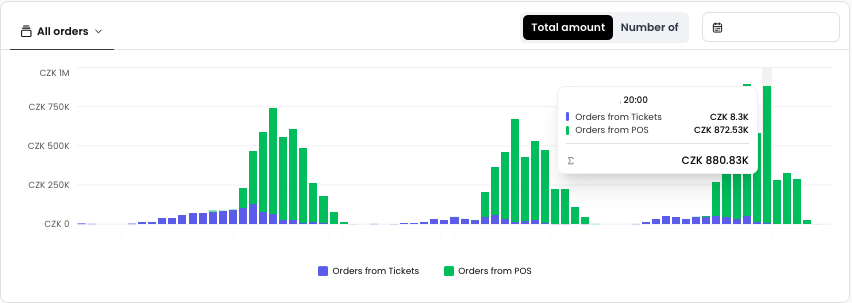
\includegraphics[width=\textwidth]{\ThesisFigures/ui/hub-chart-update}
		\caption{New Timeline Analysis in NFCtron Hub (December 2024 Update)}
		\label{fig:hub-chart-update}
		\source
	\end{figure}

	Also, thanks to the analytical findings and problems encountered during the analysis, I was able to provide valuable feedback to the development team.
	This will lead to improvements in the data collection process and the data model of the system, which will make future analysis easier and more efficient.

	Finally, the knowledge acquired by this thesis still shapes our product development and enables us to provide more advanced analytical capabilities to our clients – festival organizers.
	Future development will build upon these foundations, further expanding the analytical capabilities of NFCtron's system.
\end{section}
%%% bibliography
    \begin{flushleft}
        \bibliography{/Users/filipditrich/University/master_thesis/thesis/main,/Users/filipditrich/University/master_thesis/thesis/auto}
    \end{flushleft}
%%% list of figures
    \listoffigures
    \textit{Note: Unless stated otherwise, all figures are the author's own work.}
%%% list of tables
    \listoftables
%%% list of source codes
    \listoflistings
%%% list of abbreviations / acronyms
    %%% List of Acronyms
%%%%%%% Wording: ⏳
%%%%%%% Styling: ⏳
%%%%%%% References: ⏳
%%%%% Grammar: ⏳
%%% --------------------------------------------------------------
\chapter*{List of Acronyms}
\addcontentsline{toc}{chapter}{List of Acronyms}
\printacronyms[
    name=List of acronyms,
    heading=none,
    sort=true,
    list-style=longtable,
    extra-style=plain
]

%%% appendix
    %%% List of Appendices
%%%%%%% Wording: ✅
%%%%%%% Styling: ✅
%%%%%%% References: ✅
%%%%% Grammar: ✅
%%% --------------------------------------------------------------
\appendix
\addtocontents{toc}{\protect\setlength{\cftsecnumwidth}{22mm}}
\chapter*{List of Appendices}
\addcontentsline{toc}{chapter}{List of Appendices}
\renewcommand{\thesection}{Appendix \Alph{section}}

%%% Appendix A: Source code of the application
%%%%% File preparation: ⏳
%%%%% Instructions: ✅
%%% --------------------------------------------------------------
\begin{section}{Source code of the application}
	\label{appendix:source-code}
	The source code for the dashboard application is available on the attached CD in the~\texttt{dashboard\_app.zip} file.

	The application is built using Python 3.9\footnote{\url{https://www.python.org/downloads/release/python-390/}}, and its requirements are listed in the~\texttt{requirements.txt} file.

	The application is structured as follows:
	\begin{itemize}
		\item \texttt{app.py}: the main Dash application implementation
		\item \texttt{queries\/}: directory with SQL queries
		\item \texttt{sections\/}: directory with implementation of dashboard sections
		\item \texttt{assets\/}: directory with CSS stylesheets
		\item \texttt{\_dash\_utils.py}: utility functions for Dash
		\item \texttt{\_db\_utils.py}: common database utility functions with query manager implementation
		\item \texttt{\_query\_manager.py}: registered SQL queries
		\item \texttt{\_format\_utils.py}: utility functions for data formatting
		\item \texttt{\_chart\_utils.py}: utility functions for chart generation, SankeyDiagram implementation
	\end{itemize}

\end{section}
\newpage
%%% extended summary
    \addtocontents{toc}{\protect\contentsline{chapter}{Extended Summary}{}{}}
\end{document}
